% Template for PLoS
% Version 3.1 February 2015
%
% To compile to pdf, run:
% latex plos.template
% bibtex plos.template
% latex plos.template
% latex plos.template
% dvipdf plos.template
%
% % % % % % % % % % % % % % % % % % % % % %
%
% -- IMPORTANT NOTE
%
% This template contains comments intended 
% to minimize problems and delays during our production 
% process. Please follow the template instructions
% whenever possible.
%
% % % % % % % % % % % % % % % % % % % % % % % 
%
% Once your paper is accepted for publication, 
% PLEASE REMOVE ALL TRACKED CHANGES in this file and leave only
% the final text of your manuscript.
%
% There are no restrictions on package use within the LaTeX files except that 
% no packages listed in the template may be deleted.
%
% Please do not include colors or graphics in the text.
%
% Please do not create a heading level below \subsection. For 3rd level headings, use \paragraph{}.
%
% % % % % % % % % % % % % % % % % % % % % % %
%
% -- FIGURES AND TABLES
%
% Please include tables/figure captions directly after the paragraph where they are first cited in the text.
%
% DO NOT INCLUDE GRAPHICS IN YOUR MANUSCRIPT
% - Figures should be uploaded separately from your manuscript file. 
% - Figures generated using LaTeX should be extracted and removed from the PDF before submission. 
% - Figures containing multiple panels/subfigures must be combined into one image file before submission.
% For figure citations, please use "Fig." instead of "Figure".
% See http://www.plosone.org/static/figureGuidelines for PLOS figure guidelines.
%
% Tables should be cell-based and may not contain:
% - tabs/spacing/line breaks within cells to alter layout or alignment
% - vertically-merged cells (no tabular environments within tabular environments, do not use \multirow)
% - colors, shading, or graphic objects
% See http://www.plosone.org/static/figureGuidelines#tables for table guidelines.
%
% For tables that exceed the width of the text column, use the adjustwidth environment as illustrated in the example table in text below.
%
% % % % % % % % % % % % % % % % % % % % % % % %
%
% -- EQUATIONS, MATH SYMBOLS, SUBSCRIPTS, AND SUPERSCRIPTS
%
% IMPORTANT
% Below are a few tips to help format your equations and other special characters according to our specifications. For more tips to help reduce the possibility of formatting errors during conversion, please see our LaTeX guidelines at http://www.plosone.org/static/latexGuidelines
%
% Please be sure to include all portions of an equation in the math environment.
%
% Do not include text that is not math in the math environment. For example, CO2 will be CO\textsubscript{2}.
%
% Please add line breaks to long display equations when possible in order to fit size of the column. 
%
% For inline equations, please do not include punctuation (commas, etc) within the math environment unless this is part of the equation.
%
% % % % % % % % % % % % % % % % % % % % % % % % 
%
% Please contact latex@plos.org with any questions.
%
% % % % % % % % % % % % % % % % % % % % % % % %

\documentclass[10pt,letterpaper]{article}
\usepackage[top=0.85in,left=1.75in,footskip=0.75in]{geometry}

% Use adjustwidth environment to exceed column width (see example table in text)
\usepackage{changepage}

\usepackage{subcaption}

% Use Unicode characters when possible
\usepackage[utf8]{inputenc}

% textcomp package and marvosym package for additional characters
\usepackage{textcomp,marvosym}

% fixltx2e package for \textsubscript
\usepackage{fixltx2e}

% amsmath and amssymb packages, useful for mathematical formulas and symbols
\usepackage{amsmath,amssymb}

% cite package, to clean up citations in the main text. Do not remove.
\usepackage{cite}

% Use nameref to cite supporting information files (see Supporting Information section for more info)
\usepackage{nameref,hyperref}

% line numbers
\usepackage[right]{lineno}

% ligatures disabled
\usepackage{microtype}
\DisableLigatures[f]{encoding = *, family = * }

% rotating package for sideways tables
\usepackage{rotating}

% Remove comment for double spacing
%\usepackage{setspace} 
%\doublespacing

% Text layout
\raggedright
\setlength{\parindent}{0.5cm}
\textwidth 5.25in 
\textheight 8.75in

% Bold the 'Figure #' in the caption and separate it from the title/caption with a period
% Captions will be left justified
\usepackage[aboveskip=1pt,labelfont=bf,labelsep=period,justification=raggedright,singlelinecheck=off]{caption}

% Use the PLoS provided BiBTeX style
\bibliographystyle{plos2015}

% Remove brackets from numbering in List of References
\makeatletter
\renewcommand{\@biblabel}[1]{\quad#1.}
\makeatother

% Leave date blank
\date{}

% Header and Footer with logo
\usepackage{lastpage,fancyhdr,graphicx}
\usepackage{epstopdf}
\pagestyle{myheadings}
\pagestyle{fancy}
\fancyhf{}
\lhead{
\includegraphics[width=0.5in]{logo-main-2013.png}}
\rfoot{\thepage/\pageref{LastPage}}
\renewcommand{\footrule}{\hrule height 2pt \vspace{2mm}}
\fancyheadoffset[L]{1.25in}
\fancyfootoffset[L]{1.25in}
\lfoot{\sf csc.kth.se}

%% Include all macros below

\newcommand{\lorem}{{\bf LOREM}}
\newcommand{\ipsum}{{\bf IPSUM}}

%% END MACROS SECTION


\begin{document}
\vspace*{0.35in}

% Title must be 250 characters or less.
% Please capitalize all terms in the title except conjunctions, prepositions, and articles.
\begin{flushleft}
{\Large
\textbf\newline{Unravel motifs in UTRs and introns}
}
\newline
% Insert author names, affiliations and corresponding author email (do not include titles, positions, or degrees).
\\
Andreas Jangmo\textsuperscript{1,\Yinyang},
Johan Lord\textsuperscript{2,\Yinyang}
\\
\bigskip
\bf{1,2} Royal Institute of Technology (KTH)/School of Computer Science and Communication (CSC), Stockholm, Sweden
\bigskip

% Insert additional author notes using the symbols described below. Insert symbol callouts after author names as necessary.
% 
% Remove or comment out the author notes below if they aren't used.
%
% Primary Equal Contribution Note
\Yinyang These authors contributed equally to this work.

\end{flushleft}
% Please keep the abstract below 300 words
\section*{Abstract}
A sequence logo is a graphical representation of conserved bases in a sequence of DNA or protein. It is similar to a bar graph with the bars being stacks of letters corresponding to the nucleotides or amino acids. The logo is created from a file of aligned sequences and the size of the letters correspond to the conservation of that base at the position in the sequence specified on the x-axis. The logo can be used to illustrate a specific motif or the presence of functional units or protein binding sites in DNA sequences. In this report we have studied what the sequence logos are for the the regions before and after the translation start site and the first intron of each gene in the human genome. In doing so we first extracted the sequences for the regions of interest using Ensamble's Biomart. Using these extracted sequences we aligned them using python and created sequence logos using the python package Biopython and Weblogo. We end with a brief discussion and an interpretation of the resulting logos.

\section*{Introduction}
In genetics, a motif is a pattern in nucleotide or amino acid sequences that have, or are thought to have, a biological significance. Motifs are important as they may determine a protein's secondary structure when present in exons. It may also indicate binding sites for a large variety of proteins such as enzymes or more direct RNA level processes such as ribosome binding. Some proteins bind with very high specificity such as Type II restriction enzymes \cite{bib1}. These are part of the immune system in bacteria where they destroy viruses by splicing them up. Deviating from their binding sites could thus lead to catastrophic results. More common is that motifs vary more in composition such as the TATA box that indicates the binding site for RNA polymerase. It is apparently very rare to find a promoter that matches this sequence exactly \cite{bib1}. A convenient tool when analyzing motifs is therefore to construct something like a histogram or a bar graph illustrating the frequency of each nucleotide at each position in a region of DNA from a large number of aligned sequences. This is done by creating something called a sequence logo \cite{bib2}. A sequence logo is a graphical way of representing the variation of nucleotides or amino acids around a certain site that makes it easier to find candidate motifs. Each position relative to the site is assigned a score of information content, that is essentially a measure of the distance from a state of randomness that per definition has no information. The information content is measured in bits from complete random being 0 to perfect conservation represented by 2 bits as there are $2^2=4$ types of nucleotides. The actual letters representing the four nucleotides in our case are then scaled with their information content at each position in the sequence thus resulting a diagram called a sequence logo.

The purpose of our work has been to create sequence logos for regions in the human genome. The regions we have focused on are the ones before and after translation start site and before and after the beginning and end of the first intron of those genes that has at least one intron. Creating sequence logos for these regions might hopefully reveal conserved patterns that indicate the presence of motifs.

% You may title this section "Methods" or "Models". 
% "Models" is not a valid title for PLoS ONE authors. However, PLoS ONE
% authors may use "Analysis" 
\section*{Materials and Methods}
For the genetic information we need we have used Ensamble's Biomart \cite{bib3} mostly because of our prior knowledge of the application but also for its popularity. As a programming language we choose Python and more specifically the package Biopython \cite{bib4}. The python programs we have written and use throughout this project are \href{https://github.com/jolo2486/unravel_motifs/blob/master/bin/mergeseq.py}{mergeseq.py}, \href{https://github.com/jolo2486/unravel_motifs/blob/master/bin/cutseq.py}{cutseq.py} and \href{https://github.com/jolo2486/unravel_motifs/blob/master/bin/createlogo.py}{createlogo.py}.

\subsection*{Gathering gene data}

% For figure citations, please use "Fig." instead of "Figure".
\begin{figure}[h]
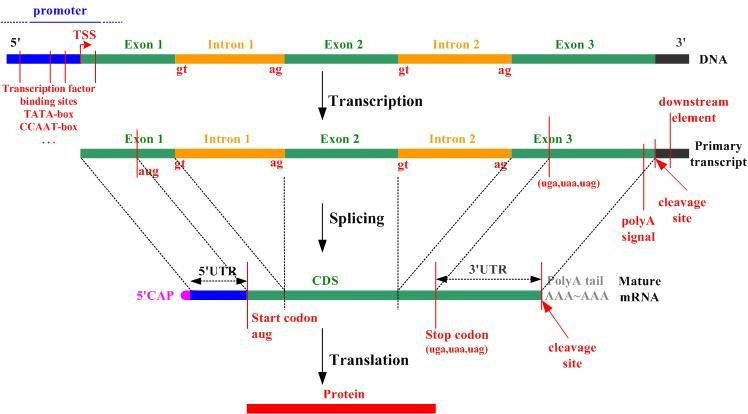
\includegraphics[width=5in]{gene_composition.jpg}
\caption{\bf An illustration of a gene showing what happens to different regions through the processes of transcription, splicing and translation.\cite{bib5}}
\label{fig1}
\end{figure}

Having decided on using as much of the human genome as possible we gathered the data using Biomart. We have used the december 2013 Homo sapiens high coverage assembly GRCh38 ("Ensambl Genes 83"/GRCh38.p5). We divided this work up into two parts: retrieving the sequences before and after the translation start site and retrieving the sequences from the beginning and end of the first intron.

Solving the first part was easy enough. From the dataset mentioned above (GRCh38.p5) we selected only coding sequences as these all start with the initiation codon. Further we added 15 nucleotides upstream to these sequences in our query to include an appropriate number of nucleotides before and after the start codon for our analysis. This was done on chromosomes 1-22, X and Y. An URL query to Biomart for this data, called Query 1, is attached as a reference \cite{bib7}.

In retrieving the introns this proved to be a bit more tedious as Biomart does not directly supply intron sequences. Studying the structure of a gene, seen in \textit{Fig} \ref{fig1}, one could though come to some conclusions. A gene include both non coding parts such as UTR:s and introns, and coding parts which consist of parts of one or more exons. Exons include the 5' and 3' UTR:s and a number of exons are spliced out to assemble a transcript which are further spliced to become a coding sequence. Thus taking the difference of the complete genes and the exons will leave the introns. As we also want to include regions upstream the start of the introns as well as downstream the end of them we achieve this by using nucleotide coordinates. This method is also convenient for other more obvious reasons as we are dealing with large amounts of data (all unspliced genes from the human genome accumulates to approx. 1.8 Gb of data). Picking out the sequences of interest by using coordinates limits the amount of data we would have to process and therefore greatly improves processing times.

We retrieved the whole unspliced genes for chromosomes 1-22, X, Y and the Exon sequences for the same using Query 2 \cite{bib8} and Query 3 \cite{bib9} respectively. The actual sequences of the exons might seem a bit redundant as we are only using the coordinates of the exons and as they are already present in the unspliced gene. However these were included for control purposes, to fail check our software and make sure it really did pick out the correct sequences as introns and exons.

\subsection*{Processing gene data}
Using the data from the previous section we now continue by filtering out the sequences to use as a base for the logo. We then need to align them in a text file in preparation for the logo creation. We implement all this using Python and the two programs doing all the work for this part are \href{https://github.com/jolo2486/unravel_motifs/blob/master/bin/mergeseq.py}{mergeseq.py} and \href{https://github.com/jolo2486/unravel_motifs/blob/master/bin/cutseq.py}{cutseq.py}.

-HIS EXCELLENCY ANDREAS CONTINUES HERE BY EXPLAINING IN MORE DETAIL ABOUT OUR ALGORITHM FOR THIS-

\subsection*{Creating sequence logos}
For sequence logo creation there are a few tools at our disposal. We choose to use Steven Brenner's WebLogo \cite{bib6} for its simplicity and the possibility of accessing this tool via the function weblogo() in the Biopython class motifs. Weblogo is mainly used through their web application which we initially used for experimental purposes. It can also be used by downloading their source code, by using their python package or from a third party software such as Biopython. We choose to implement this using the above mentioned function weblogo() in Biopython. Weblogo uses a multiple sequence alignment as a basis for logo creation. Three file formats for these alignments are available: FASTA, ClustalW and Flat. Flat format means that the sequences are just listed on top of each other without sequence names or other header information. Since we had no use for header information at this point, flat format was definitely most suited for our purposes. The simplicity of the flat format also made scripting a bit simpler.

Using the flat formatted alignment files created in the previous step a python program called \href{https://github.com/jolo2486/unravel_motifs/blob/master/bin/createlogo.py}{createlogo.py} goes through each line of the file and adds that sequence as a Biopython Seq object to a list. From this list a Biopython motif object is created and from this object the logo is created by connecting to the weblogo service via the function weblogo() in the motifs class. Thus one needs an internet connection to use this program. The output of createlogo.py is simply a PNG file displaying the logo.

% Results and Discussion can be combined.
\section*{Results and Discussion}
The three resulting logos from the region around the start codon and around the beginning and end of the first intron can be seen in \textit{Fig} \ref{fig2}. For the logo of the region around the start codon there did not seem to be any easy way to ignore the start codon (as this obviously blows up) so we choose to show it as it is but adjusted the y axis to show more information of the other areas.

% CHANGE FILENAME OF THE PICTURE IN THIS FIGURE
\begin{figure}[h]
\begin{subfigure}{.5\textwidth}
  \centering
  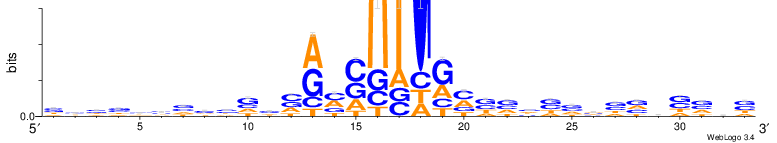
\includegraphics[width=5in]{../../results/2016-01-04/coding_sequences_logo.png}
  \caption{}
  \label{fig:sfig1}
\end{subfigure}%

\begin{subfigure}{.5\textwidth}
  \centering
  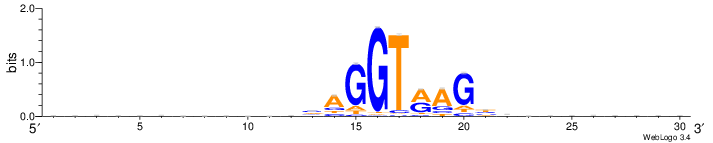
\includegraphics[width=5in]{../../results/2016-01-04/usg_intr_1_us_15.png}
  \caption{}
  \label{fig:sfig2}
\end{subfigure}

\begin{subfigure}{.5\textwidth}
  \centering
  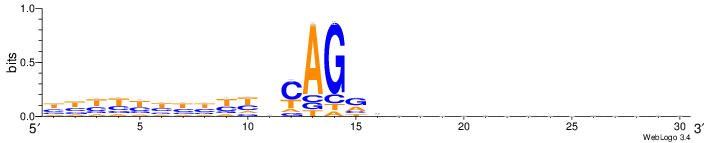
\includegraphics[width=5in]{../../results/2016-01-04/usg_intr_1_ds_15.png}
  \caption{}
  \label{fig:sfig2}
\end{subfigure}
\caption{\bf (a) The logo for the sequence 15 nucleotides upstream to 15 nucleotides downstream the initiation codon. (b) The logo for the sequence 15 nucleotides upstream to 15 nucleotides downstream the start of the first intron. (c) The logo for the sequence 15 nucleotides upstream to 15 nucleotides downstream the end of the first intron.}
\label{fig2}
\end{figure}

As we can see in \ref{fig:sfig1}, GCC and ACC seems higly conserved right before the start and G seems to be conserved directly after it. This is quite expected as it agrees with a well known consensus sequence found in eukaryotic mRNA known as the Kozak sequence \cite{bib10}, after Marilyn Kozak. This has the consensus (gcc)gccRccAUGG where R stands for a purine (A or G). The Kozak sequence is not the same as the ribosomal binding site but is recognized by the ribosome and plays a huge role in the initiation of translation.

-FILL IN MORE SMART CONCLUSIONS AND LOUD FABULOUS DISCUSSIONS HERE-

\subsection*{\lorem\ and \ipsum\ Nunc blandit a tortor.}

Maecenas convallis mauris sit amet sem ultrices gravida. Etiam eget sapien nibh. Sed ac ipsum eget enim egestas ullamcorper nec euismod ligula. Curabitur fringilla pulvinar lectus consectetur pellentesque. Quisque augue sem, tincidunt sit amet feugiat eget, ullamcorper sed velit. Sed non aliquet felis. Lorem ipsum dolor sit amet, consectetur adipiscing elit. Mauris commodo justo ac dui pretium imperdiet. Sed suscipit iaculis mi at feugiat. 

\subsection*{Sed ac quam id nisi malesuada congue.}

Nulla mi mi, venenatis sed ipsum varius, volutpat euismod diam. Proin rutrum vel massa non gravida. Quisque tempor sem et dignissim rutrum. Lorem ipsum dolor sit amet, consectetur adipiscing elit. Morbi at justo vitae nulla elementum commodo eu id massa. In vitae diam ac augue semper tincidunt eu ut eros. Fusce fringilla erat porttitor lectus cursus, vel sagittis arcu lobortis. Aliquam in enim semper, aliquam massa id, cursus neque. Praesent faucibus semper libero.

% Please do not create a heading level below \subsection. For 3rd level headings, use \paragraph{}. 
\subsection*{Subsection 1}
Nulla mi mi, venenatis sed ipsum varius, volutpat euismod diam. Proin rutrum vel massa non gravida. Quisque tempor sem et dignissim rutrum. Lorem ipsum dolor sit amet, consectetur adipiscing elit. Morbi at justo vitae nulla elementum commodo eu id massa. In vitae diam ac augue semper tincidunt eu ut eros. Fusce fringilla erat porttitor lectus cursus, vel sagittis arcu lobortis. Aliquam in enim semper, aliquam massa id, cursus neque. Praesent faucibus semper libero.

\subsection*{Subsection 2}
\paragraph{3rd Level Heading.} Nulla mi mi, venenatis sed ipsum varius, volutpat euismod diam. Proin rutrum vel massa non gravida. Quisque tempor sem et dignissim rutrum. Lorem ipsum dolor sit amet, consectetur adipiscing elit. Morbi at justo vitae nulla elementum commodo eu id massa. In vitae diam ac augue semper tincidunt eu ut eros. Fusce fringilla erat porttitor lectus cursus, vel sagittis arcu lobortis. Aliquam in enim semper, aliquam massa id, cursus neque. Praesent faucibus semper libero.

\section*{Acknowledgments}
Cras egestas velit mauris, eu mollis turpis pellentesque sit amet. Interdum et malesuada fames ac ante ipsum primis in faucibus. Nam id pretium nisi. Sed ac quam id nisi malesuada congue. Sed interdum aliquet augue, at pellentesque quam rhoncus vitae.

\nolinenumbers

%\section*{References}
% Either type in your references using
% \begin{thebibliography}{}
% \bibitem{}
% Text
% \end{thebibliography}
%
% OR
%
% Compile your BiBTeX database using our plos2015.bst
% style file and paste the contents of your .bbl file
% here.
% 
\begin{thebibliography}{10}

\bibitem{bib1}
D'haeseleer Patrik, What are DNA sequence motifs? Nature Biotechnology 24, 423 - 425 (2006)

\bibitem{bib2}
Schneider, T.D. \& Stephens, R.M. Sequence Logos: a new way to display consensus sequences. Nucleic Acids Res. 18, 6097–6100 (1990).

\bibitem{bib3}
Ensembl release 83, December 2015 © WTSI / EMBL-EBI
http://www.ensembl.org/index.html

\bibitem{bib4}
Biopython 1.66, released on 21 October 2015.
http://biopython.org/wiki/Main\_Page

\bibitem{bib5}
Prof B. Jayaram \& Co-workers, Genome Tutorials. Supercomputing Facility for Bioinformatics \& Computational Biology, IIT Dehli.
As of 2016-01-03 avaible here:
http://www.scfbio-iitd.res.in/research/genomics.html

\bibitem{bib6}
Crooks GE, Hon G, Chandonia JM, Brenner SE WebLogo: A sequence logo generator, Genome Research, 14:1188-1190, (2004)

\bibitem{bib7}
Query 1: Coding sequences for chromosome 1-22, X, Y with 15 nucleotides upstream flank, Header: Gene ID, Ensembl release 83, December 2015 © WTSI / EMBL-EBI

\url{http://www.ensembl.org/biomart/martview/e8279e04f1de2a2309c53c23a7a5aa05?VIRTUALSCHEMANAME=default&ATTRIBUTES=hsapiens_gene_ensembl.default.sequences.ensembl_gene_id|hsapiens_gene_ensembl.default.sequences.coding|hsapiens_gene_ensembl.default.sequences.upstream_flank."15"&FILTERS=hsapiens_gene_ensembl.default.filters.chromosome_name."1,2,3,4,5,6,7,8,9,10,11,12,13,14,15,16,17,18,19,20,21,22,X,Y"&VISIBLEPANEL=resultspanel}

\bibitem{bib8}
Query 2: Unspliced gene for chromosome 1-22, X, Y, Headers: Gene ID, gene start, gene end, Ensembl release 83, December 2015 © WTSI / EMBL-EBI

\url{http://www.ensembl.org/biomart/martview/e8279e04f1de2a2309c53c23a7a5aa05?VIRTUALSCHEMANAME=default&ATTRIBUTES=hsapiens_gene_ensembl.default.sequences.ensembl_gene_id|hsapiens_gene_ensembl.default.sequences.start_position|hsapiens_gene_ensembl.default.sequences.end_position|hsapiens_gene_ensembl.default.sequences.gene_exon_intron&FILTERS=hsapiens_gene_ensembl.default.filters.chromosome_name."1,2,3,4,5,6,7,8,9,10,11,12,13,14,15,16,17,18,19,20,21,22,X,Y"&VISIBLEPANEL=resultspanel}

\bibitem{bib9}
Query 3: Exon sequences for chromosome 1-22, X, Y, Headers: Gene ID, exon start, exon end, strand, Ensembl release 83, December 2015 © WTSI / EMBL-EBI

\url{http://www.ensembl.org/biomart/martview/e8279e04f1de2a2309c53c23a7a5aa05?VIRTUALSCHEMANAME=default&ATTRIBUTES=hsapiens_gene_ensembl.default.sequences.ensembl_gene_id|hsapiens_gene_ensembl.default.sequences.gene_exon|hsapiens_gene_ensembl.default.sequences.exon_chrom_start|hsapiens_gene_ensembl.default.sequences.exon_chrom_end|hsapiens_gene_ensembl.default.sequences.strand&FILTERS=hsapiens_gene_ensembl.default.filters.chromosome_name."1,2,3,4,5,6,7,8,9,10,11,12,13,14,15,16,17,18,19,20,21,22,X,Y"&VISIBLEPANEL=resultspanel}

\bibitem{bib10}
Kozak, M (31 January 1986). "Point mutations define a sequence flanking the AUG initiator codon that modulates translation by eukaryotic ribosomes.". Cell 44 (2): 283–92

\end{thebibliography}



\end{document}

